\documentclass[11pt]{article}
\usepackage[utf8]{inputenc}
\usepackage[T1]{fontenc}
\usepackage[british]{babel}
\usepackage{hyperref}
\usepackage{graphicx}
\usepackage{natbib}
\usepackage{tikz}
\usetikzlibrary{positioning, arrows.meta}
\usepackage{float} 

\begin{document}
\begin{titlepage}
    \centering
    \includegraphics[scale=0.1]{uu.jpg}\par\vspace{1cm}
    {\large \textbf{Introduction to ES/CS Work Group 3 Project Report}\par}
    {\Huge \textbf{Pi-Streamer}\par}
    \vspace{1cm}
    {\Large Tejas Chakravarthy, Andreas Hadjoullis, Sarafroz Bekmurodova, Hardik Sai Kotagiri\par}
    \vfill
    {\large \ 10th October 2025\par}
\end{titlepage}


\begin{abstract}
This project presents the design and implementation of a lightweight video streaming system that enables users to upload, transcode, and playback media content through a web interface. The main objective was to develop a working prototype demonstrating adaptive streaming using open-source technologies and a modular architecture suitable for educational and small-scale deployment. 

The project was built using a Flask-based backend for handling file uploads and API requests, an FFmpeg-based transcoding pipeline for segmenting and encoding video into HTTP Live Streaming (HLS) format, and finally a frontend for browser-based playback. All components were deployed using a Raspberry Pi distribution of the Linux operating system and using standard HTTP delivery without external dependencies. 

The implemented solution successfully demonstrates real-time conversion of uploaded videos into multi-resolution HLS streams accessible via a web player. The project demonstrates how modern media protocols and free software can be used to create a functional streaming workflow, providing a foundation for future extensions such as live streaming, authentication, or cloud-based scalability. Given the limitations of the Raspberry Pi, the project demonstrates simple functionality.
\end{abstract}

\tableofcontents

\section{Introduction}
In recent years, the proliferation of compact, low-cost computing platforms such as the Raspberry Pi has significantly broadened opportunities for experimentation in applied computer science. These platforms provide sufficient computational power to implement distributed systems, network services, and lightweight applications, while remaining accessible to students and researchers. This project investigates the design and implementation of a multimedia streaming service hosted on a Raspberry Pi, with the aim of understanding both the technical processes involved and the collaborative practices required to deliver a functioning system.

The project is situated within the broader context of online video consumption, where streaming has become the predominant medium. Large-scale providers such as Netflix and YouTube employ sophisticated architectures that ensure adaptive resolution, low latency, and high availability. By contrast, this project explores whether similar principles can be achieved on a constrained platform using only open-source software and modest resources. The exercise therefore serves not only as a technical prototype, but also as a means of learning about software integration, system configuration, and cross-platform accessibility.

Equally central to the project is the process of teamwork and knowledge sharing. Our group adopted a rotating role model in which members alternated as coordinator, developer, tester, and documentation writer. This arrangement ensured that responsibilities were distributed equitably, that all members were exposed to different aspects of the project, and that collaboration was reinforced through regular communication. Progress was tracked through scheduled milestones, allowing us to assess whether the system was developing in line with expectations.

The report documents both technical achievements and reflections on the collaborative process. Specifically, it describes the research and methodological choices underlying the implementation, the ethical considerations of deploying a streaming service, and the lessons learned during development. The structure of the report is as follows: section 2 surveys related work and comparable implementations. Section 3 presents the methodological framework guiding the project. Section 4 considers ethical questions relevant to the design and deployment of streaming technologies. Section 5 outlines the details of the implementation, including architectural decisions and testing procedures. Section 6 summarises team contributions and role allocation. Finally, we conclude with section 7.

\section{Background / Related Work}
Streaming media technologies have undergone a series of evolutionary stages, beginning with file download-and-playback approaches and progressing towards adaptive streaming protocols that dominate contemporary usage. Initial attempts to improve interactivity and reduce latency, such as the Real Time Streaming Protocol (RTSP), provided a foundation for streaming but were hindered by compatibility issues and limited scalability. The subsequent emergence of HTTP-based streaming marked a turning point, allowing video segments to be delivered over standard web infrastructure.

Among the most influential protocols is HTTP Live Streaming (HLS)\cite{apple_hls}, introduced by Apple, which divides video into small segments and provides adaptive bitrate switching. Its counterpart, MPEG-DASH, similarly enables adaptive streaming over HTTP, with comparable advantages in compatibility and scalability. Both approaches exploit existing Content Delivery Networks (CDNs), minimising deployment overhead.

Implementation tools have also matured. The open-source utility \texttt{ffmpeg} has become the standard for video transcoding, capable of converting raw video into multiple formats and resolutions. In parallel, lightweight web servers such as \texttt{nginx} have demonstrated reliability in serving large numbers of concurrent requests. When combined, these tools provide a practical framework for hosting adaptive streaming services on modest hardware.

Within the academic literature, research on multimedia streaming highlights trade-offs between quality, compression, and latency. Fielding’s \cite{fielding2000} work on architectural styles remains influential in framing discussions of scalability and modularity in distributed systems. Further studies emphasise the increasing demand for adaptive methods that respond to heterogeneous devices and variable network conditions.

At the level of educational practice, projects involving Raspberry Pi streaming are not uncommon. Prior initiatives have demonstrated the feasibility of using the device as a media centre or a server for small-scale deployments. However, relatively few projects integrate these technical exercises with structured reflections on teamwork, project management, and ethical responsibility. This report therefore positions itself at the intersection of technical exploration and collaborative learning.

\section{Methods}

\begin{figure}[H]
\centering
\resizebox{0.95\textwidth}{!}{%
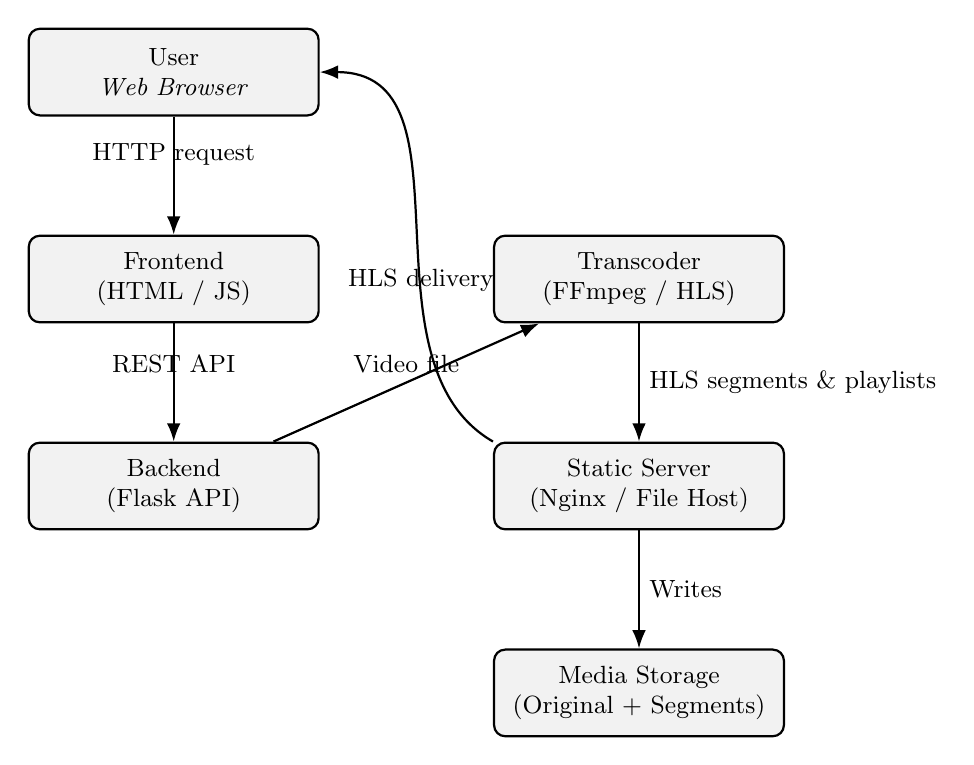
\begin{tikzpicture}[
    >=Latex,
    node distance=1.5cm and 2.2cm,
    every node/.style={font=\small, align=center},
    box/.style={
        draw, rounded corners, thick, fill=gray!10,
        minimum height=1.1cm, text width=3.4cm, inner sep=4pt
    },
    line/.style={-Latex, thick}
]

% --- Left column: User + Frontend + Backend (vertical stack) ---
\node[box] (user) {User\\\textit{Web Browser}};
\node[box, below=of user] (frontend) {Frontend\\(HTML / JS)};
\node[box, below=of frontend] (backend) {Backend\\(Flask API)};

% --- Right column: Transcoder + Server + Storage (vertical stack) ---
\node[box, right=of frontend] (ffmpeg) {Transcoder\\(FFmpeg / HLS)};
\node[box, below=of ffmpeg] (server) {Static Server\\(Nginx / File Host)};
\node[box, below=of server] (storage) {Media Storage\\(Original + Segments)};

% --- Connections with labels placed to avoid overlap ---
\draw[line] (user) -- node[pos=0.5, above]{HTTP request} (frontend);
\draw[line] (frontend) -- node[pos=0.5, above]{REST API} (backend);
\draw[line] (backend) -- node[pos=0.5, above]{Video file} (ffmpeg);
\draw[line] (ffmpeg) -- node[pos=0.5, right]{HLS segments \& playlists} (server);
\draw[line] (server) -- node[pos=0.5, right]{Writes} (storage);

% Curved return path to the user with label outside nodes
\draw[line] (server.north west) to[out=150, in=0]
    node[pos=0.35, above]{HLS delivery} (user.east);

\end{tikzpicture}%
}
\caption{Overall system architecture showing interaction between client, frontend, backend, transcoding, storage, and content delivery.}
\label{fig:architecture}
\end{figure}

\subsection{Methodology} The methodological approach combined structured planning, iterative development, and reflective evaluation. At the outset, the group established a contract defining rotating roles, conflict resolution strategies, and communication channels. Progress checkpoints were agreed upon, including deadlines for research, environment setup, implementation, and testing. Meetings were held at regular intervals to monitor progress and adjust the plan where necessary.

\subsection{Research and Design.} The group reviewed available tools for video transcoding, web serving, and user interface development. Alternatives such as GStreamer or VLC were considered, but ffmpeg was selected due to its maturity, documentation, and flexibility. Nginx was chosen as the primary web server, and Python-based web development tools were identified as the most appropriate means of producing a landing page for user access. This decision reflected both familiarity within the group and the suitability of Python for rapid prototyping.

\subsection{Environment Setup.} The Raspberry Pi was prepared with a suitable Raspberry Pi Linux operating system and network configuration. This was selected and used for open-source accessibility and package integration. Package dependencies for ffmpeg, nginx, and Python libraries were installed from freely available open-source repositories. This ensured that no software was restricted or was required to be purchased for the project. Accessibility testing was then integrated into this stage to ensure that the service could be reached from both desktop and mobile devices. A high level design of the environment can be seen in the figures~\ref{fig:architecture} and~\ref{fig:workflow}.



%\section{Implementation Activities.} Tasks were distributed according to role. The developer focused on configuring ffmpeg and nginx, the coordinator worked on the Python-based landing page, the tester ensured cross-platform accessibility, and the documentation writer maintained the evolving report draft.

\begin{figure}[H]
\centering
\resizebox{0.95\textwidth}{!}{%
\begin{tikzpicture}[
    node distance=1.6cm and 1.8cm,
    every node/.style={font=\small, align=center},
    step/.style={draw, rounded corners, thick, fill=blue!10, minimum width=3.0cm, minimum height=1.0cm},
    arrow/.style={-Latex, thick}
]

% --- Top row ---
\node[step] (upload)    {1. User\\uploads video};
\node[step, right=of upload] (save) {2. Backend\\stores file};
\node[step, right=of save] (transcode) {3. FFmpeg\\transcodes \& segments};

% --- Bottom row ---
\node[step, below=of save] (playlist) {4. HLS playlists\\generated};
\node[step, right=of playlist] (playback) {5. HTML5 player\\requests HLS};

% --- Flow arrows ---
\draw[arrow] (upload) -- (save);
\draw[arrow] (save) -- (transcode);
\draw[arrow] (transcode) |- (playlist);
\draw[arrow] (playlist) -- (playback);

\end{tikzpicture}%
}
\caption{Sequential workflow of video processing and playback in the system.}
\label{fig:workflow}
\end{figure}

\subsection{Testing and Evaluation.} Transcoding was validated through playback of different videos. The HLS playlist was inspected for correctness, and nginx logs were reviewed for error handling. Accessibility tests verified that media could be streamed through both local and wireless networks. Later tests introduced HTTPS certificates to ensure secure connections.

\subsection{Reflection and Adjustment.} Throughout the process, the group evaluated outcomes in light of objectives. Hardware acceleration was attempted but limited by the Raspberry Pi’s performance. Difficulties with certificate configuration delayed the introduction of HTTPS, but these obstacles ultimately reinforced understanding of security protocols.

\section{Ethical Considerations}
Although the project did not involve human subjects, it engaged several ethical dimensions that required careful reflection.

First, streaming technologies inherently raise questions of copyright and content ownership. The group elected to use only openly licensed or self-produced media files to avoid potential infringement. This decision ensured that the prototype demonstrated functionality without contravening intellectual property law.

Second, privacy and security considerations shaped system design. Because the system operated as a network-accessible service, precautions were taken to restrict deployment to controlled environments. HTTPS encryption was configured to prevent interception of data in transit. These measures align with broader ethical imperatives to protect user privacy and prevent misuse of technology.

Third, the use of artificial intelligence tools in the preparation of the report was explicitly limited in accordance with institutional guidelines. Language models were used solely for spelling and grammar checking, with all substantive content generated and critically reviewed by the group members. This ensured both originality and academic integrity.

Finally, the collaborative dimension of the project required adherence to ethical standards of fairness and transparency. Rotating roles and a conflict resolution procedure were introduced to prevent unequal distribution of labor and to manage potential disagreements constructively. Although conflicts did not arise, the framework reinforced accountability and trust within the group.

In our case we approach ethics using the 'ethical egotism' framework, since we prioritize our need/desire to stream content, over the concern of copyrighted content and piracy issues.

\section{Implementation}
\subsection{Technical Overview.}
\subsubsection{Architecture.}
The system is a small LAN media streaming service running on a Raspberry Pi. The three main components are: (1) an HTTP server (nginx) that serves static HLS content (.m3u8 playlists and .ts segments), (2) a lightweight Python backend (Flask)\cite{flask_quickstart} that accepts uploads, stores originals, schedules transcoding using ffmpeg and exposes a small API, and (3) a client-side frontend (single-page UI + a standalone player) that uploads media, lists available items and plays HLS streams. This separation keeps playback fast and simple (nginx serves static files) while Flask handles control, metadata and the CPU-intensive transcoding jobs.

\subsubsection{Server and filesystem layout.}
All web content and HLS output are placed under a single web root: \\/var/www/pi\_streamer/media. Within that directory we keep original/ (uploaded source files), hls/<id>/ (transcoded HLS outputs for each media item), and static frontend files (index.html, player.html, styles.css, script.js). Nginx is configured to serve /hls/ from the hls subfolder and to proxy small API calls (/api/*) to the Flask process on 127.0.0.1:8080. File and directory permissions are set so the nginx user can read and write to the directories directly.

\subsubsection{Media processing (FFmpeg -> HLS).}
When a user uploads a file the backend saves the original to original/ and schedules a background transcode job. Our chosen workflow transcodes on upload (pre-generate HLS) because it provides predictable playback and avoids CPU spikes at first play. FFmpeg is used to produce HLS VOD output: a playlist (playlist.m3u8) and fixed-length segment files (segment\_000.ts, segment\_001.ts, …)\cite{ffmpeg_hls}. The FFmpeg command preserves the input resolution. Typical FFmpeg options used are -c:v libx264 -preset veryfast -crf 23 and -c:a aac -b:a 128k with -hls\_time 6 and -hls\_list\_size 0 for VOD. Due to storage limitations on the raspberry Pi and development issues, we chose not to go through with multiple resolutions for each video uploaded. Meaning, the content will be stream-able only in its original resolution.

\subsubsection{Backend design and job orchestration.}
The backend is a single-file Flask app with a tiny SQLite metadata store (media.db). Endpoints include POST /api/upload (accept file upload), GET /api/media (list media), GET /api/status/<id> (status), and /watch/<id> (redirect to the HLS playlist). Uploads are validated (secure\_filename, extension checks) and saved with a UUID to avoid collisions. A ThreadPoolExecutor (configured with a low max\_workers to protect the Pi’s CPU, e.g., 1) runs FFmpeg tasks asynchronously so the upload response can return immediately with a status URL. The DB stores status transitions: queued -> processing -> ready | failed and the frontend polls the API to show progress.

\subsubsection{Nginx configuration highlights.}
Nginx\cite{nginx_static} is configured to: (1) serve static HLS content and player assets from /var/www/pi\_streamer/media, (2) set correct MIME types for .m3u8 and .ts, (3) add permissive CORS headers during development (Access-Control-Allow-Origin: *) so mobile/desktop browsers can fetch segments, and (4) increase client\_max\_body\_size and adjust timeouts to allow large uploads (e.g., client\_max\_body\_size 2048M). The server block also proxies /api/ and /watch/ to the Flask backend and returns standard access/error logs for debugging.

\subsubsection{Frontend (index + player).}
The frontend is intentionally minimal and dependency-light. index.html (plus styles.css and index.js) provides an upload form with an XHR-based uploader that shows a progress bar, a media library rendered from /api/media, and an “Open in player” link which redirects to player.html. player.html is a small standalone page that reads ?id=<id> from the URL, constructs /hls/<id>/playlist.m3u8, and streams the video. If the browser supports native HLS (Safari) video.src is set to the .m3u8. Otherwise, hls.js\cite{hls-js} is used.

\subsection{Results.}
\subsubsection{Deployment decisions, limitations and future work.}
For the one-month project scope we run nginx + ffmpeg + Flask on the Pi host. This is robust for small LAN demos with a few simultaneous viewers. Limitations: CPU and storage constraints on the Pi make multi-bitrate live transcoding expensive. Future improvements that would enhance the project: generate automatic thumbnails, offer multiple resolutions for each video, and establish a publicly available domain.

\subsubsection{Security.} HTTPS certificates were installed to provide encrypted connections, enhancing trust and preventing potential interception. The topic was difficult to research, as there  is a large number of options to choose from. In the end, for the sake of simplicity, we chose \texttt{mkcert}. The program was used to create 
certificates for our local website, and then nginx was configured to use said certificates.

\subsubsection{Testing and Performance.} The system was tested on both desktop and mobile clients, including access via local hotspots. Playback was evaluated for latency and stability. The system functioned reliably for demonstration purposes as can be seen from the results on figure~\ref{fig:test-results}.

\begin{figure}[H]
    \centering
    %\hspace*{-6cm}                                                           
    \includegraphics[width=1\linewidth]{test-results.jpeg}
    \caption{Test results}
    \label{fig:test-results}
\end{figure}

\subsection{General Challenges.}
One of the main challenges in this project was the effort required to properly integrate several different software components into a single working system. While tools like Nginx, FFmpeg, Flask, and hls.js each serve a clear purpose, bringing them together highlighted many small incompatibilities and configuration details that were not immediately obvious from the start. Documentation was often fragmented, meaning we had to spend significant time searching through examples, community forums, and official manuals to understand how each tool should be configured in the context of our project. Setting up Nginx was particularly challenging, as its directory structure and default configuration varied between Linux distributions. On our system, our custom configuration would not take effect until we explicitly removed the pre-installed “default” server block, which otherwise took priority and returned 404 errors. These integration issues ultimately improved our understanding of how the underlying components fit together.

As mentioned before, even though originally we had intentions of generating multiple resolutions for each video, ultimately we decided not to, for the following reasons:
\begin{itemize}
    \item the storage space on our raspberry Pi was strictly limited to 16GB, thus this idea was deemed as a poor usage of our resources
    \item generating multiples playlists and syncing them through a master playlist was very error prone and consistently caused bugs
\end{itemize}

\subsection{Summary.}
The implemented system is a practical, end-to-end HLS streaming prototype: users can upload files via a simple frontend, the backend transcodes and produces HLS content with FFmpeg, nginx serves the static HLS artifacts to any device on the LAN, and the client UI supports standalone playback with cross-browser compatibility using the native HLS + hls.js fallback pattern. The design prioritizes simplicity, reproducibility and clarity while leaving clear paths for performance hardening and feature expansion. The end result of our implementation is shown in figures~\ref{fig:pi-streamer-homepage} and ~\ref{fig:pi-streamer-playerpage}.

\begin{figure}[H]
    \centering
    \includegraphics[width=2\linewidth]{pi-streamer-homepage.png}
    \caption{Pi-Streamer Homepage}
    \label{fig:pi-streamer-homepage}
\end{figure}
\begin{figure}[H]
    \centering
    \hspace*{-6cm}                                                           
    \includegraphics[width=2\linewidth,]{pi-streamer-playerpage.png}
    \caption{Pi-Streamer Player page}
    \label{fig:pi-streamer-playerpage}
\end{figure}

\section{Contributions}
Each member contributed to all aspects of the project, but specific responsibilities were distributed as follows:

\textbf{Tejas Chakravarthy (Coordinator):} Coordinated group activities, ensured adherence to milestones, and contributed to development of the Python-based landing page. Drafted sections of the report, particularly on methodology and introduction.


\textbf{Andreas Hadjoullis (Developer):} Implemented ffmpeg integration with nginx, configured HLS streaming, and attempted hardware acceleration. Documented technical aspects of the system architecture.

\textbf{Hardik Sai (Tester):} Conducted extensive testing across platforms, validated HTTPS configuration, and reported on playback performance. Assisted in final evaluation and refinement.

\textbf{Sarafroz Bekmurodova (Documentation Writer):} Drafted the report in LaTeX, synthesised related work, and ensured citation consistency. Supported interface evaluation and coordinated proofreading.

All members engaged in research, implementation, and preparation of the final presentation. Communication was maintained through online platforms, and a clear conflict resolution protocol was established, though not required. The balanced distribution of tasks reinforced fairness and provided all members with experience across different aspects of the project lifecycle.

\section{Conclusion}
In this project we successfully implemented a media streaming service hosted on a Raspberry Pi, combining Nginx, FFmpeg, Flask, and hls.js into a working system. Users can upload media files, which are processed into HLS format and securely streamed over HTTPS to a variety of client devices. While we faced challenges with integration, configuration, and adapting to differences across environments, these difficulties provided valuable hands-on experience with networking, web servers, and media handling. Overall, the project not only met its technical goals but also deepened our practical understanding of building and deploying networked applications.

\section{Reference List}
\bibliographystyle{ieeetr}
\begin{thebibliography}{9}

\bibitem{apple_hls}
Apple Inc.
\newblock {HTTP Live Streaming — Apple Developer Documentation}.
\newblock \url{https://developer.apple.com/documentation/http-live-streaming}.
\newblock Accessed: 14 October 2025.

\bibitem{fielding2000}
Roy T. Fielding.
\newblock {Architectural Styles and the Design of Network-based Software Architectures}.
\newblock PhD thesis, University of California, Irvine, 2000.
\newblock Accessed: 14 October 2025.

\bibitem{ffmpeg_hls}
FFmpeg Developers.
\newblock {FFmpeg Formats Documentation (HLS muxer)}.
\newblock \url{https://ffmpeg.org/ffmpeg-formats.html}.
\newblock Accessed: 14 October 2025.

\bibitem{flask_quickstart}
Pallets.
\newblock {Flask Documentation (3.1.x): Quickstart}.
\newblock \url{https://flask.palletsprojects.com/en/stable/quickstart/}.
\newblock Accessed: 14 October 2025.

\bibitem{nginx_static}
NGINX, Inc.
\newblock {Beginner’s Guide — Serving Static Content}.
\newblock \url{https://nginx.org/en/docs/beginners_guide.html}.
\newblock Accessed: 14 October 2025.

\bibitem{hls-js}
hls.js
\newblock {hls.js Github}.
\newblock \url{https://github.com/video-dev/hls.js/}.
\newblock Accessed: 14 October 2025.

\end{thebibliography}

\end{document}
